\section{Model 2}

The results displayed in this section are for the uncertainty involved in the calculation of flamespeed depending  on two parameter i.e the activation energy for the fall off reaction in the ozone mechanism and activation energy for second reaction in the mechanism. The percentage of ozone is taken as 40, 46, 53, 75, and 100  percent according to the experimental data available to us from Streng\cite{Streng}. In the
figure~\ref{subfig-4:KDE_21},  we display results for sample size 1e7 and surrogate
of 100X100 points.  We show the the KDE for parameters $E_2$ and $E_3$.

\bigskip

In the figure~\ref{subfig-1:E2_sample_conv} and figure~\ref{subfig-1:E3_sample_conv} , for
constant surrogate size of 100x100, the number of samples are changed from 1e5 to
1e7 and convergence is observed. The plot is done for raw chain size of $1e5$, $5e5$ , $1e6$, $5e6$ and $1e7$ is taken. In the figure~\ref{subfig-1:E2_surrogate_conv} and figure~\ref{subfig-1:E3_surrogate_conv},
convergence study is done for surrogates with differing number of interpolation points. As we increase the number of points in the surrogate, results should be close for different surrogate sizes. The plot is done for surrogate size of 10X10, 20X20 30X30 , 100X100, 150X150 and 200X200 for both parameters $E_2$ and $E_3$. In this analysis, raw sample chain size is $1e6$. For different starting points of MCMC chain, the MAP point of the resulting pdf does not change. The surrogates for individual concentrations are constructed using linear interpolation
function. The initial guess for the MAP point is calculated using Nelder Mead optimization technique. 


\bigskip

In the
figure~\ref{subfig-1:mean_2} and figure~\ref{subfig-2:autocorr_2},  mean and correlation plots are shown for
the samples of the parameters $E_2$ and $E_3$. The mean plot shows the initial instability due to sum in period of MCMC and after that it remains constant. It shows us that we should be using at least more than these number of samples for our analysis. The figure~\ref{subfig-1:e2_distribution_2} shows the posterior of the parameter $E_2$ with the following parameters of the distribution- :Mean:  18.9, Std. Dev.:  4.77, Skewness:  -1.38 and Kurtosis:  4.55.  The figure~\ref{subfig-1:e3_distribution_2} shows the posterior of the parameter $E_3$ with the following parameters of the distribution- Mean:  11.7, Std. Dev.: 7.81, Skewness:  -0.743 and Kurtosis:  1.29.


The results are displayed in five sections. In first section, the plots are shown for kernel density estimation of parameters $E_3$ and $E_2$. In second section, for constant surrogate size, the number of samples are changed from 1e5 to 1e7 and convergence is observed. In the third part of the results, convergence study is done for surrogates with different sizes. In fourth section, we ensure that samples of the parameter which we are drawing are fitting the flamespeed values of the experiment. In the fifth section mean and correlation plots are shown for the samples of both the parameters. The surrogates for individual concentrations are constructed using linear interpolation function. The initial guess for the map point is calculated using nelder mead optimization technique. After supplying initial guess over large domain it is found that the map point is the same no matter where we start our guess.


\bigskip

 It is necessary to ensure that the samples of the parameter which we are drawing are fitting the flamespeed values of the experiment. In the figure~\ref{subfig-1:40_2}, figure~\ref{subfig-2:46_2}, figure~\ref{subfig-3:53_2}, figure~\ref{subfig-4:75_2}, and figure~\ref{subfig-5:100_2},   we calculate the flamespeed for all the parameters drawn using the surrogate generated before for 40$\%$, 46$\%$, 53$\%$, 75$\%$, and 100 $\%$ respectively. We have taken $1e7$ sample size and calculated flamespeed for all the concentrations of ozone mentioned. We have a good fit to the data overall.

%\subsection{ Statistics }

% In this section, we display results for sample size 1e7 and surrogate of 100X100 points. We  have plotted the KDE



%\subsection{Convergence Study: Number of Samples }

% In this section, we see the convergence of the probability distribution as we increase the raw chain sample size. The plot is done for surrogate size of 100. In this analysis, raw chain size of $1e5$, $5e5$ , $1e6$, $5e6$ and $1e7$ is taken.




%\subsection{Convergence Study: Surrogate }

%In this section, we see the convergence of the surrogate. As we increase the number of points in the surrogate, results should be close for different surrogate sizes. The plot is done for surrogate size of 10X10, 20X20 30X30 , 100X100, 150X150 and 200X200. In this analysis, raw sample chain size is $1e6$.



%\subsection{Flamespeed data Fit}

 %It is necessary to ensure that the samples of the parameter which we are drawing are fitting the flamespeed values of the experiment. In this section, we calculate the flamespeed for all the parameters drawn using the surrogate generated before. We have taken $1e7$ sample size and calculated flamespeed for different concentrations of ozone.





%\subsection{Mean and Autocorrelation Plots}

%In this section, we show the mean of the samples and autocorrelation plots . The mean plot shows the initial instability due to burning period of MCMC and after that it remains constant. It shows us that we should be using atleast more than these number of samples for our analysis. The last figure shows the histogram and the various parameters of the distribution. For E3: Mean:  11.7, Std. Dev.: 7.81, Skewness:  -0.743 and Kurtosis:  1.29. For E2 stats:Mean:  18.9, Std. Dev.:  4.77, Skewness:  -1.38 and Kurtosis:  4.55.




\begin{figure}[H]
\centering
\subfloat[KDE \label{subfig-4:KDE_21}]{
        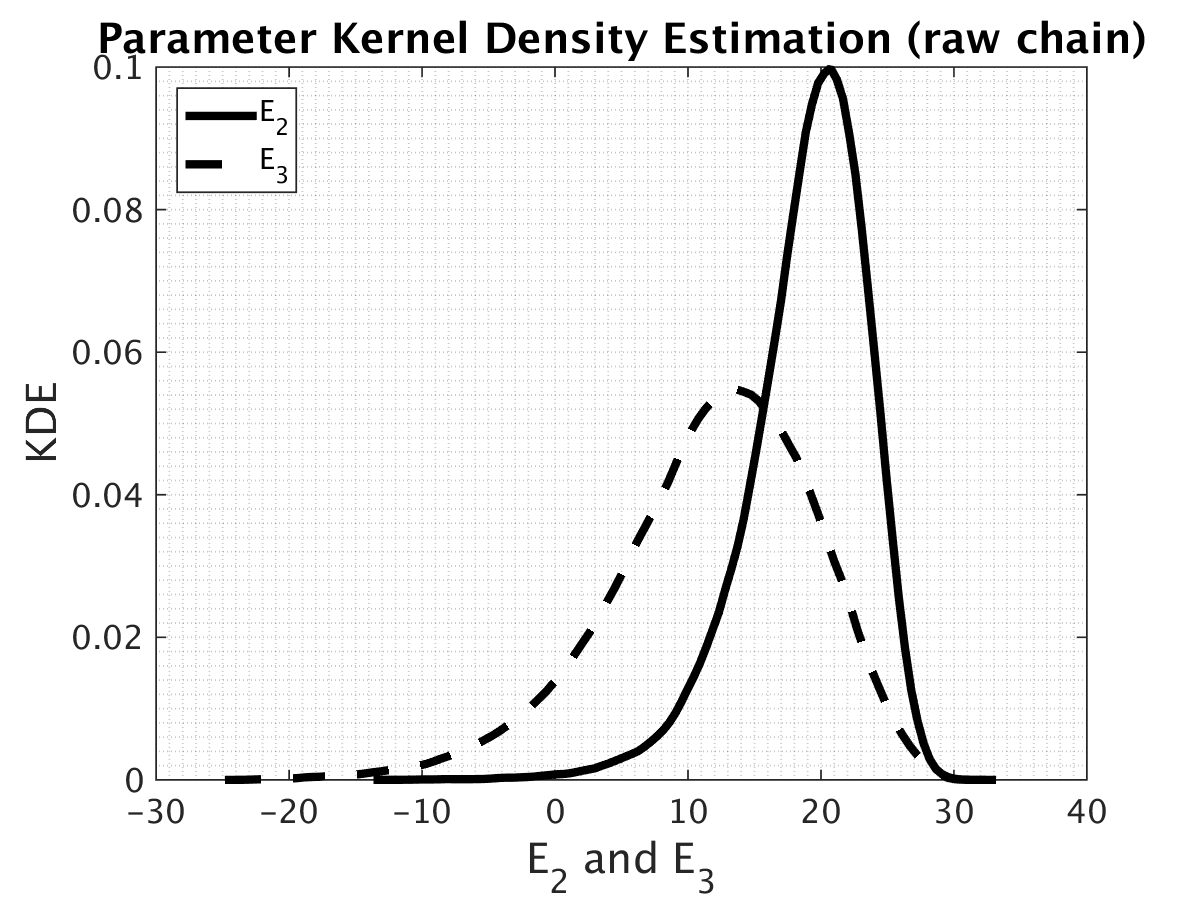
\includegraphics[scale=0.7]{model_2/kde}
            }
    \caption{Results for sample size 1e7}
\end{figure}

\begin{figure}[H]
\subfloat[Convergence For $E_2$ \label{subfig-1:E2_sample_conv}]{
        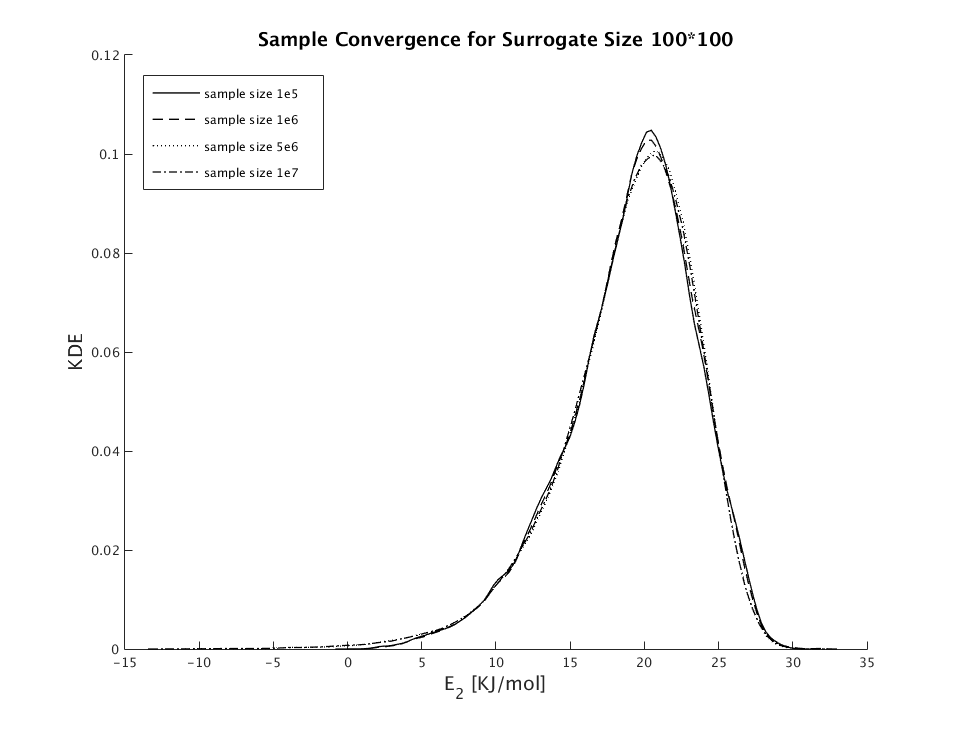
\includegraphics[scale=0.3]{model_2/sample_conv_E2}
            }
 \subfloat[Convergence For $E_3$ \label{subfig-1:E3_sample_conv}]{
        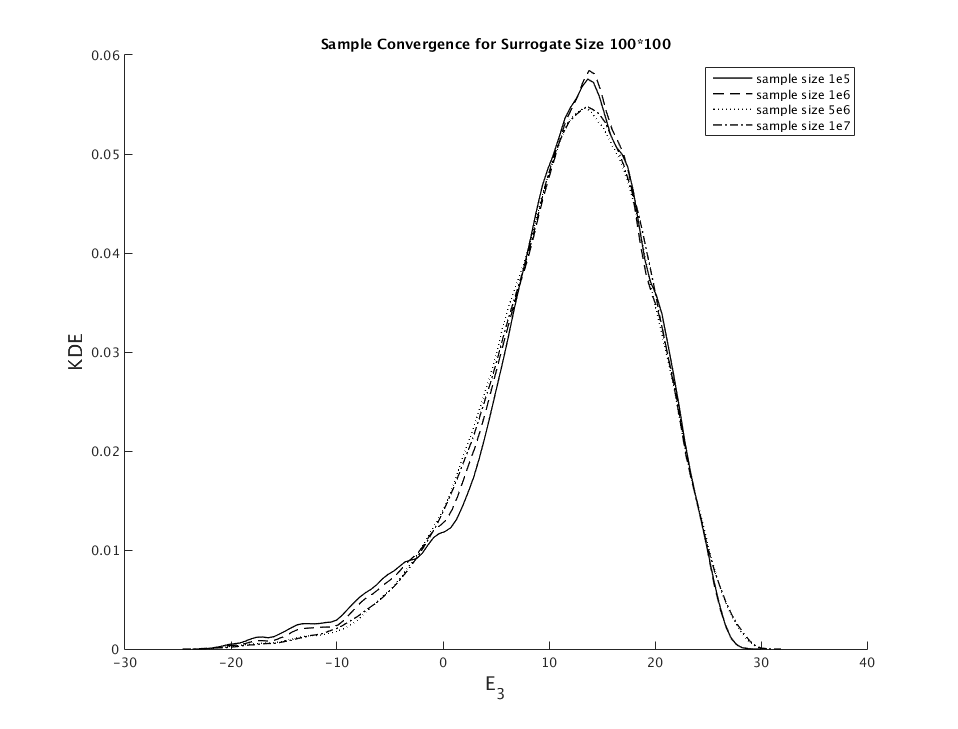
\includegraphics[scale=0.3]{model_2/sample_conv_E3}
            }
            \caption{Convergence with respect to sample size}
\end{figure}

\begin{figure}[H]
\subfloat[Surrogate Convergence For $E_2$ \label{subfig-1:E2_surrogate_conv}]{
        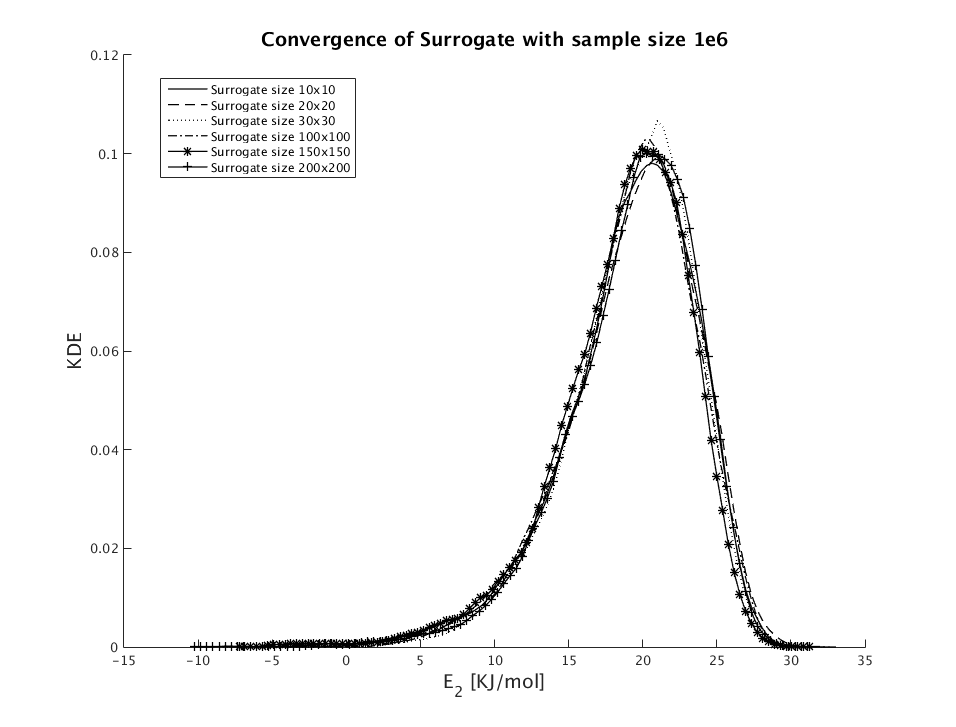
\includegraphics[scale=0.3]{model_2/surrogate_conv_E2}
            }
 \subfloat[ Surrogate Convergence For $E_3$ \label{subfig-1:E3_surrogate_conv}]{
        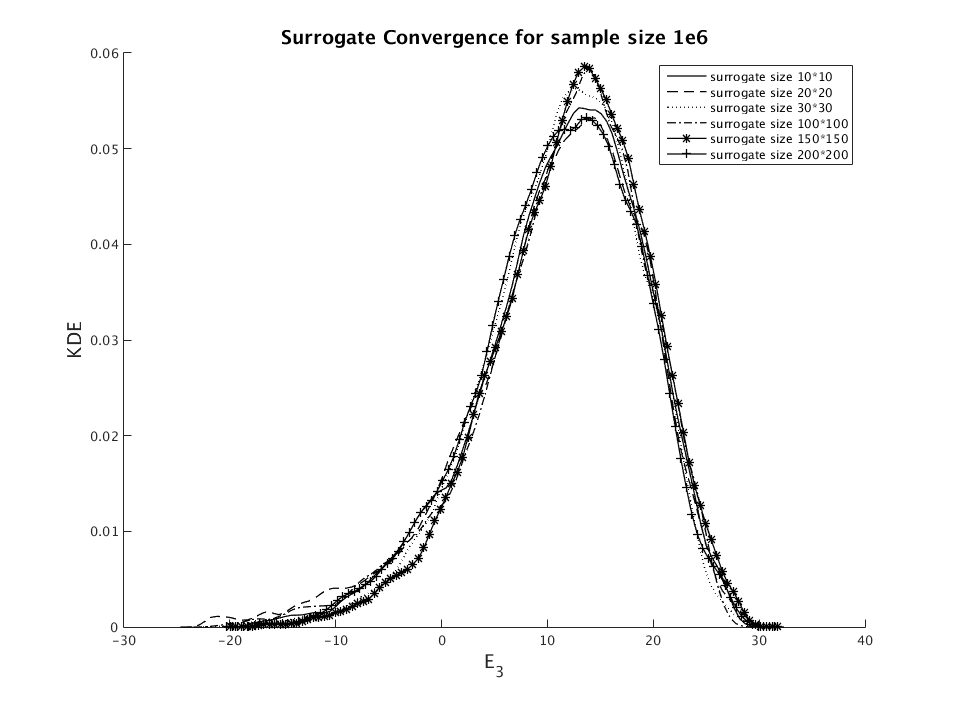
\includegraphics[scale=0.3]{model_2/surrogate_conv_E3}
            }
            \caption{Convergence with respect to number of surrogate points}
\end{figure}

 \begin{figure}[H]
   \subfloat[ Flame speed for 40 \% ozone \label{subfig-1:40_2}]{
        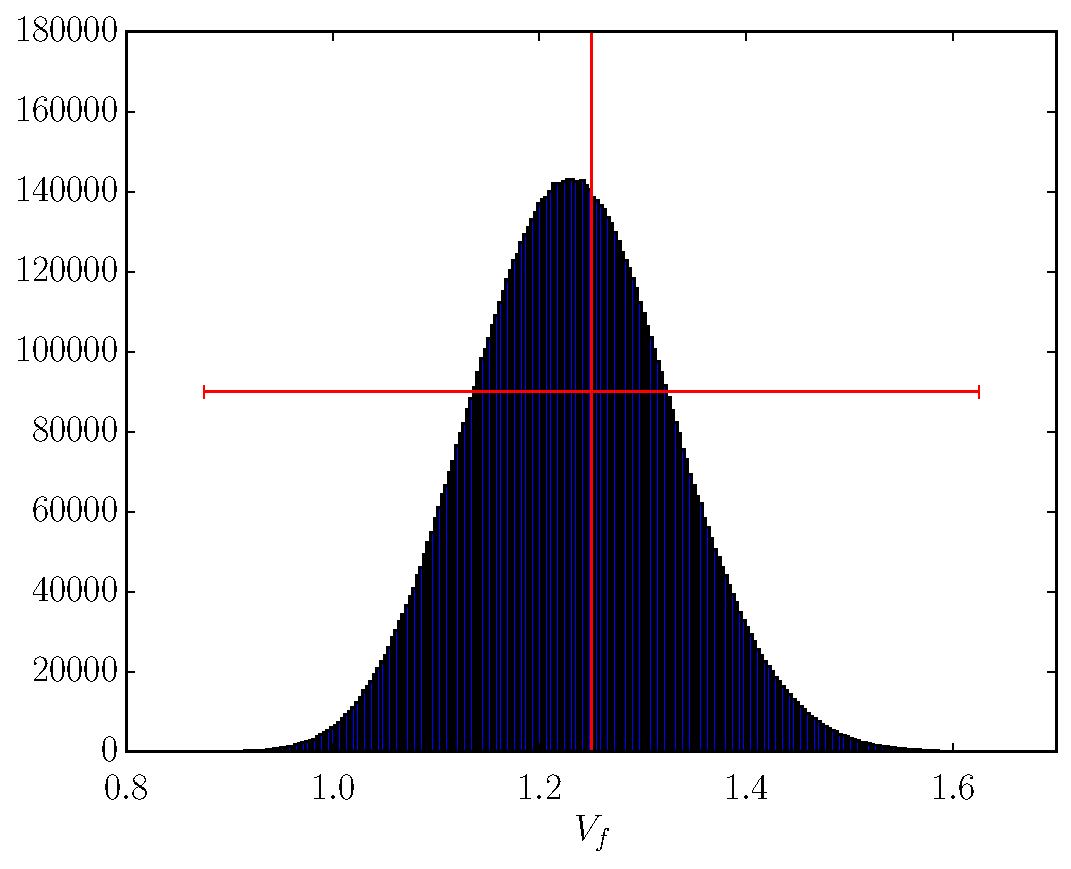
\includegraphics[scale=0.45]{model_2/flame_40.pdf}
       }
\subfloat[Flame speed for 46 \% ozone \label{subfig-2:46_2}]{
        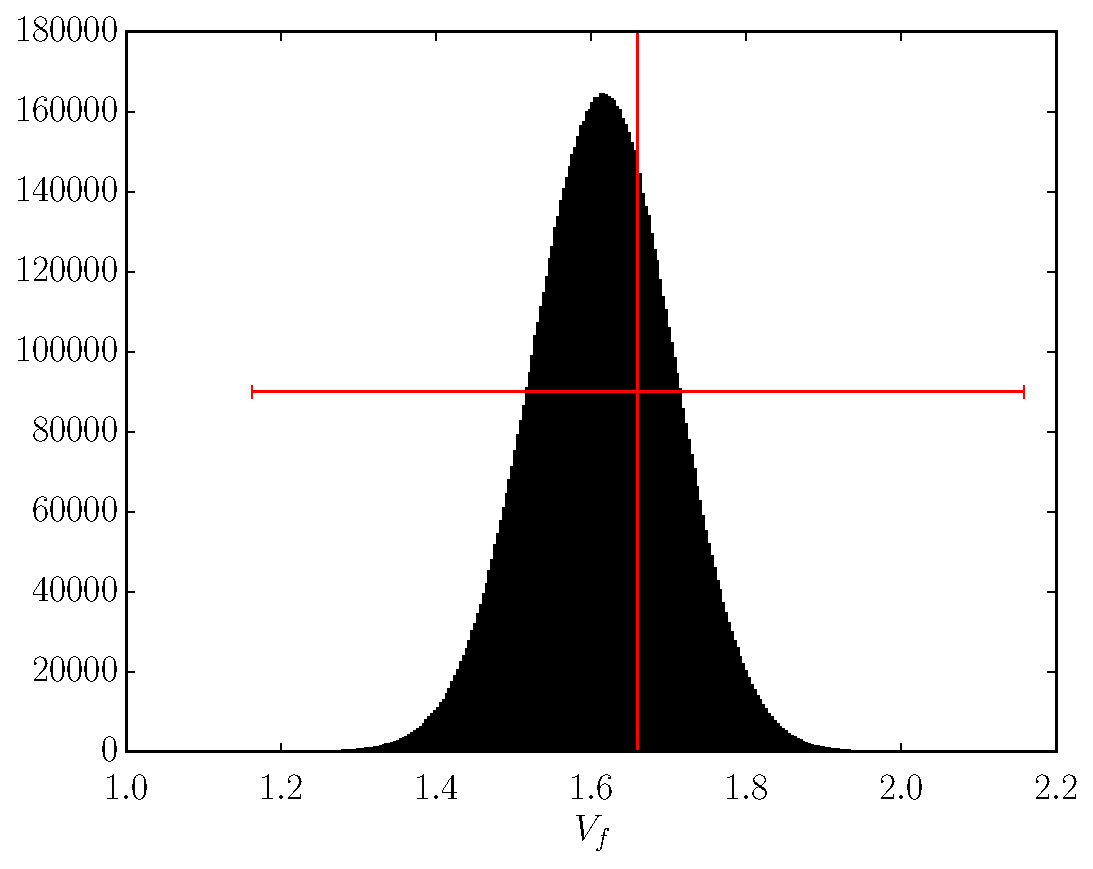
\includegraphics[scale=0.45]{model_2/flame_46.pdf}
            }
\end{figure}


 \begin{figure}[H]
  \ContinuedFloat
   \subfloat[ Flame speed for 53 \% ozone \label{subfig-3:53_2}]{
        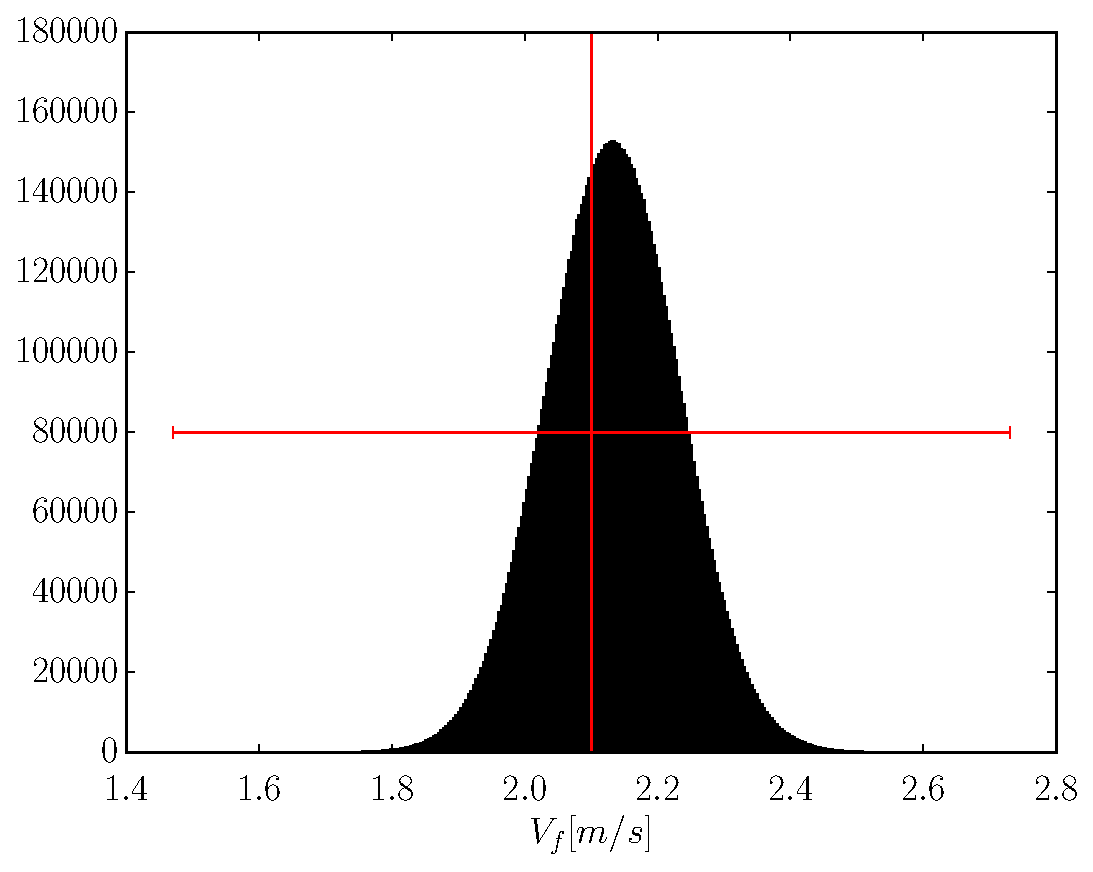
\includegraphics[scale=0.45]{model_2/flame_53.pdf}
       }
\subfloat[Flame speed for 75 \% ozone \label{subfig-4:75_2}]{
        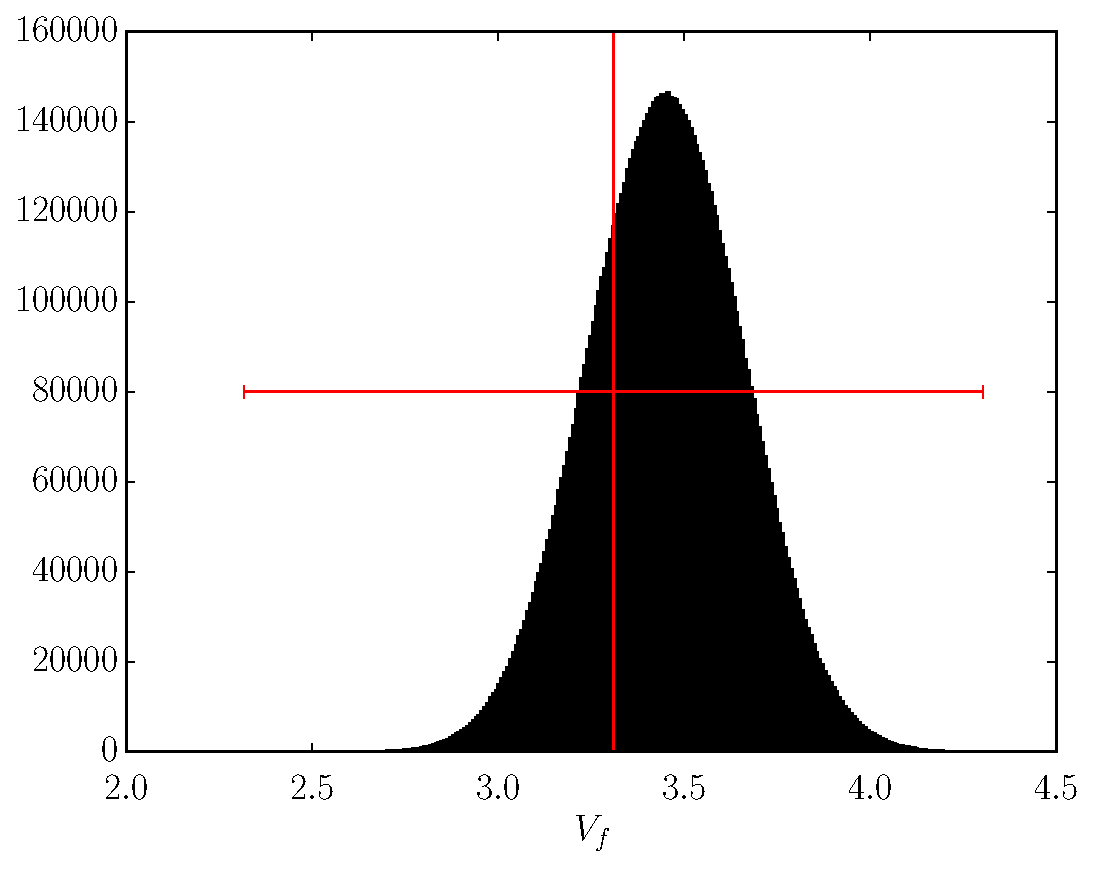
\includegraphics[scale=0.45]{model_2/flame_75.pdf}
            }
\end{figure}


 \begin{figure}[H]
  \ContinuedFloat
   \subfloat[ Flame speed for 100 \% ozone \label{subfig-5:100_2}]{
        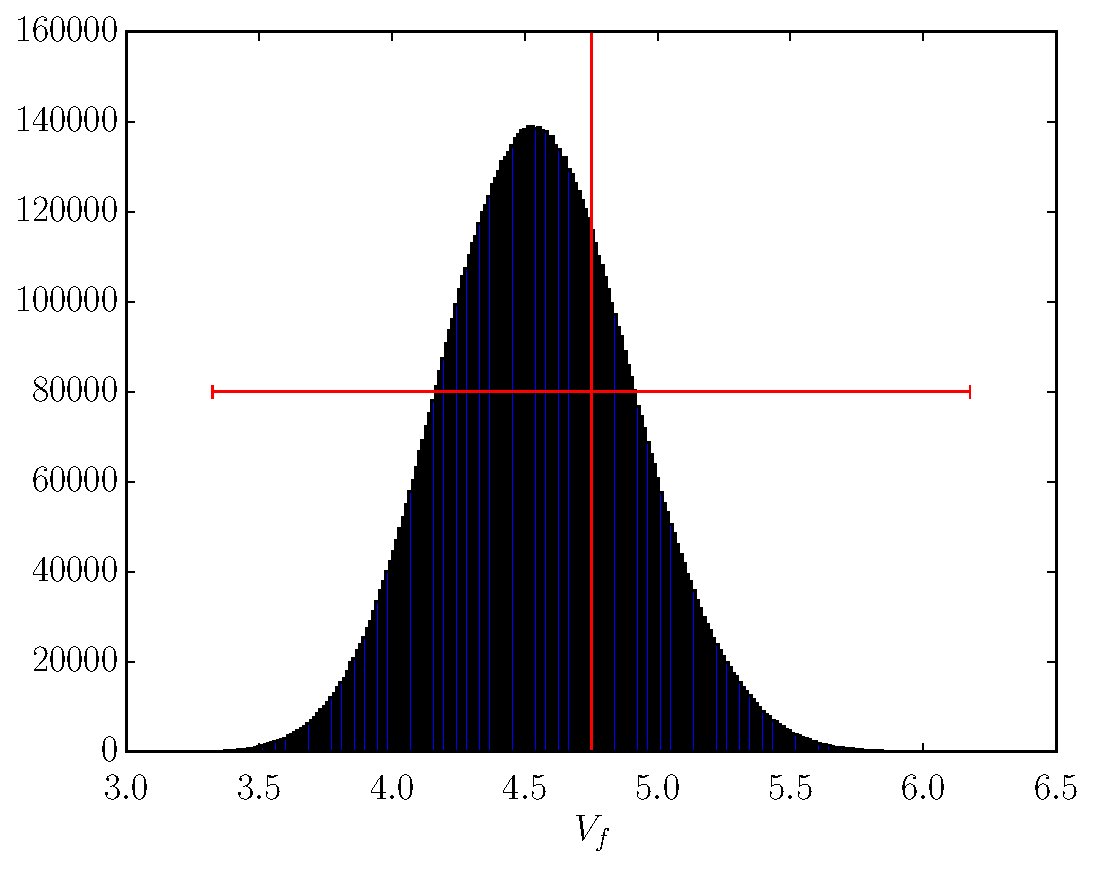
\includegraphics[scale=0.45]{model_2/flame_100.pdf}
       }
  \caption{Flamespeed Data fit}
\end{figure}


 \begin{figure}[H]
   \subfloat[ Mean \label{subfig-1:mean_2}]{
        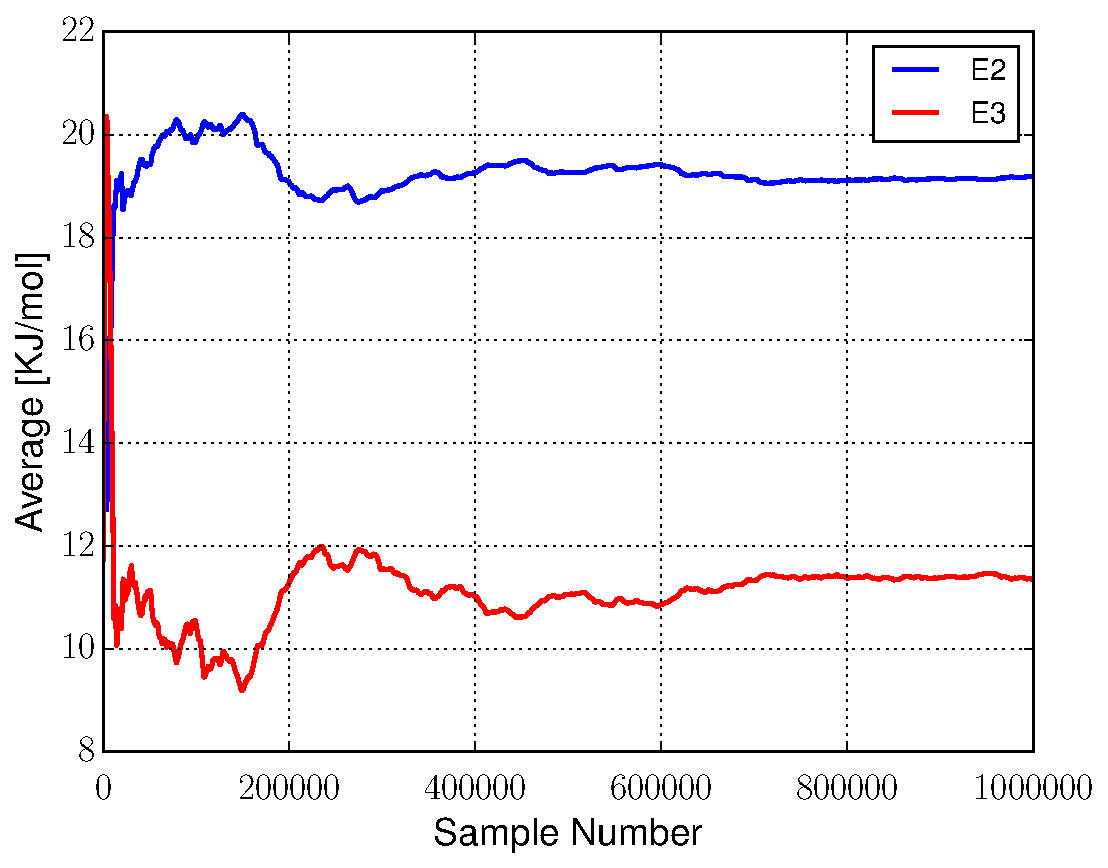
\includegraphics[scale=0.45]{model_2/M1_running_avg.pdf}
       }
\subfloat[Autocorrelation \label{subfig-2:autocorr_2}]{
        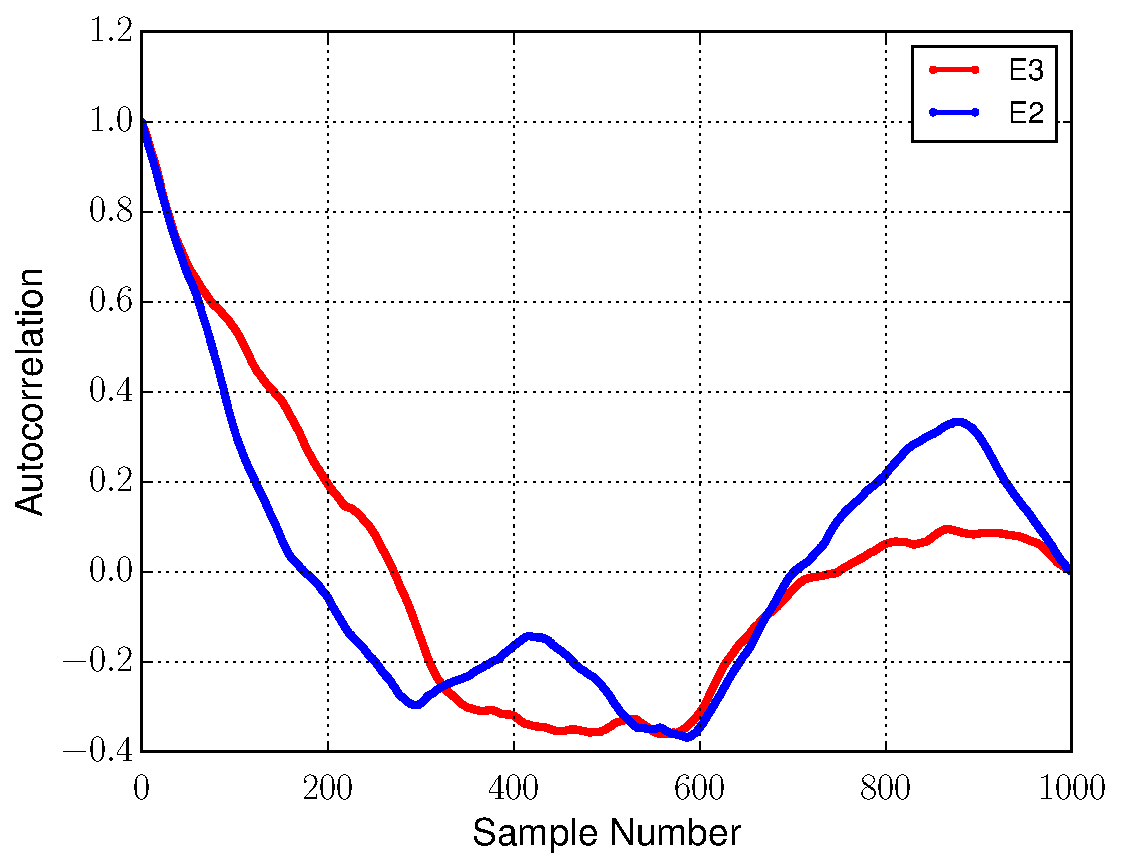
\includegraphics[scale=0.45]{model_2/M1_autocorr.pdf}
            }
            \caption{Mean and autocorrelation for sample size 1e6}
\end{figure}

 \begin{figure}[H]      
\subfloat[  $E_2$ distribution  \label{subfig-1:e2_distribution_2}]{
        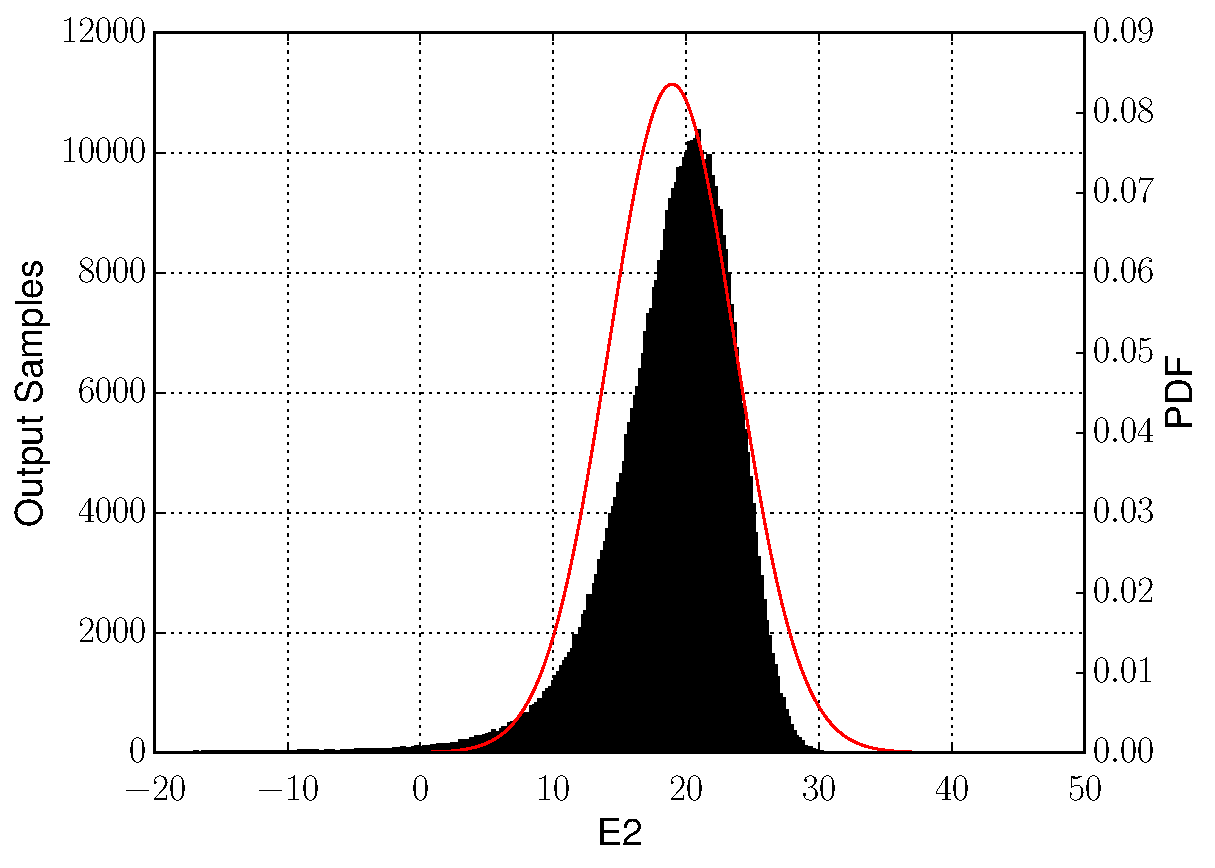
\includegraphics[scale=0.43]{model_2/E2.pdf} 
            }  
 \subfloat[ $E_3$ distribution  \label{subfig-1:e3_distribution_2}]{
        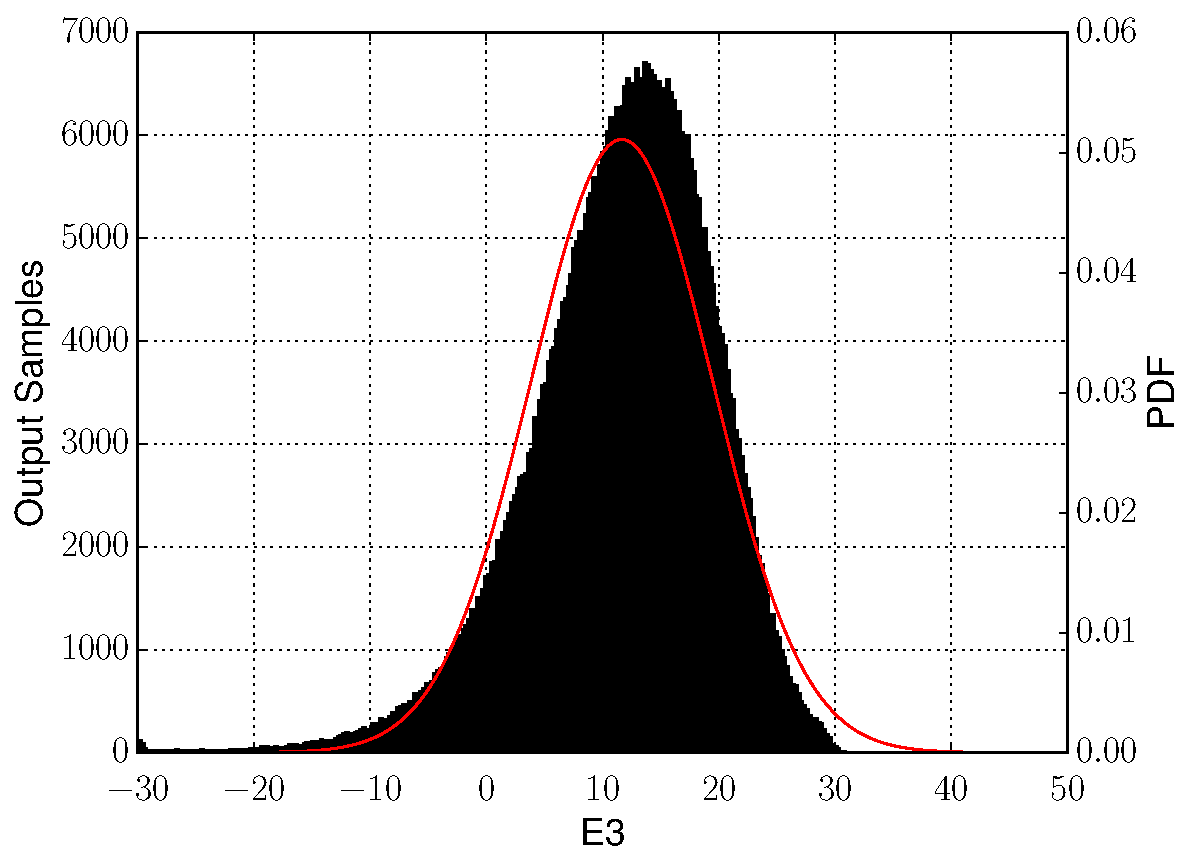
\includegraphics[scale=0.43]{model_2/E3.pdf}
            }
            \caption{$E_3$ and $E_2$ posterior distributions}
\end{figure}
